\tikzset{
   plane/.pic = {
    \draw[fill]  plot[smooth, tension=0.6] coordinates {
        (-0.65,-0.9) 
        (-0.6,-0.85) 
        (-0.4,-0.75) 
        (-0.25,-0.65) 
        (-0.15,-0.5) 
        (-0.12,-0.3) 
        (-0.1,-0.1) 
        (0,0) 
        (0.1,-0.1) 
        (0.12,-0.3) 
        (0.15,-0.5) 
        (0.25,-0.65) 
        (0.4,-0.75) 
        (0.6,-0.85) 
        (0.65,-0.9)
        } -- plot[smooth, tension=0.6] coordinates {
        (0.65,-0.9) 
        (0.15,-0.91)
        (0.35,-1.1) 
        (0.37,-1.15)
        } -- plot[smooth, tension=0.6] coordinates {
        (0.37,-1.15)
        (0,-1.12) 
        (-0.37,-1.15) 
        } -- plot[smooth, tension=0.6] coordinates {
        (-0.37,-1.15)
        (-0.35,-1.1) 
        (-0.15,-0.91) 
        (-0.65,-0.9) 
        } -- cycle;
   }
}
\newcommand{\rvec}[1]{\ensuremath{{\boldsymbol{\underline{#1}}}}}
\newcommand{\rv}[1]{\ensuremath{{\boldsymbol{#1}}}}
\newcommand{\mat}[1]{{\ensuremath{{\mathbf{#1}}}}}

\usetikzlibrary{math}

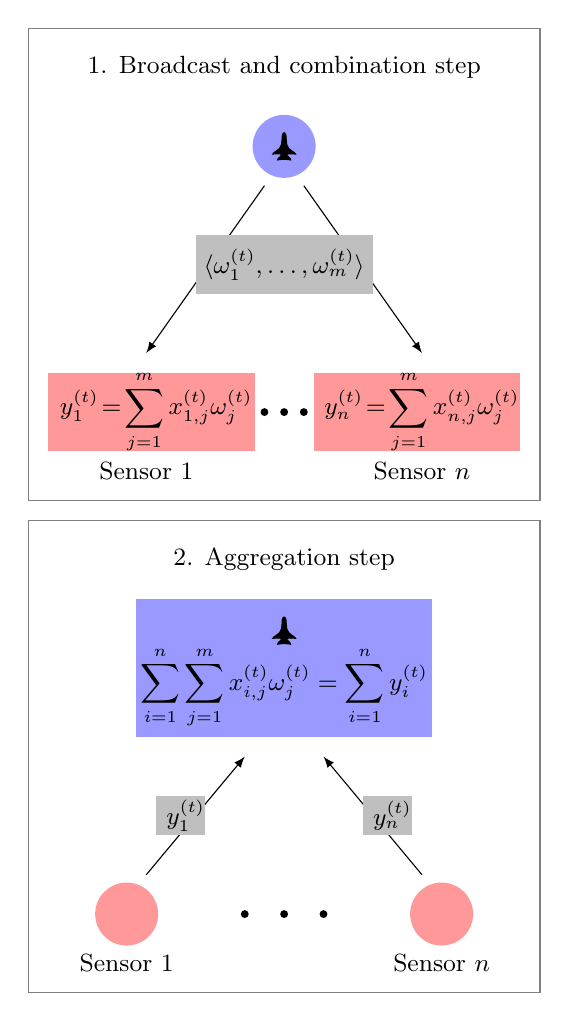
\begin{tikzpicture}[font=\small]
    % Step 1
    \node at (3.25,5.5) {1. Broadcast and combination step};
    % Navigator
    \fill (3.25,4.5) [blue!40] ellipse (0.4 and 0.4);
    \pic[xscale=0.22,yscale=0.3] at (3.25,4.6725) {plane};
    % Sensors
    \node at (1.5,0.375) {Sensor $1$};
    \fill [red!40] (0.25,0.625) rectangle (2.875,1.625);
    \node at (1.625,1.125) {$\displaystyle y_1^{(t)} \!=\! \sum^m_{j=1}x_{1,j}^{(t)}\omega_j^{(t)}$};
    \node at (5,0.375) {Sensor $n$};
    \fill [red!40] (3.625,0.625) rectangle (6.25,1.625);
    \node at (5,1.125) {$\displaystyle y_n^{(t)} \!=\! \sum^m_{j=1}x_{n,j}^{(t)}\omega_j^{(t)}$};
    \fill [black] (3.5,1.125) circle (0.05);
    \fill [black] (3,1.125) circle (0.05);
    \fill [black] (3.25,1.125) circle (0.05);
    % Lines
    \draw [-latex] plot[smooth, tension=.7] coordinates {(3.5,4) (5,1.875)};
    \draw [-latex] plot[smooth, tension=.7] coordinates {(3,4) (1.5,1.875)};
    \fill [lightgray] (2.125,3.375) rectangle (4.375,2.625);
    \node at (3.25,3) {$\langle\omega_1^{(t)},\dots ,\omega_m^{(t)}\rangle$};
    
    % Step 2
    \node at (3.25,-0.75) {2. Aggregation step};
    % Navigator
    \fill [blue!40] (1.375,-3) rectangle (5.125,-1.25);
    \pic[xscale=0.22,yscale=0.3] at (3.25,-1.4775) {plane};
    \node at (3.25,-2.375) {$\displaystyle \sum^{n}_{i=1}\sum^{m}_{j=1} x_{i,j}^{(t)}\omega_j^{(t)} = \sum^n_{i=1}y^{(t)}_{i}$};
    % Sensors
    \node at (1.25,-5.875) {Sensor $1$};
    \fill  (5.25,-5.25) [red!40] ellipse (0.4 and 0.4);
    \node at (5.25,-5.875) {Sensor $n$};
    \fill  (1.25,-5.25) [red!40] ellipse (0.4 and 0.4);
    \fill [black] (2.75,-5.25) circle (0.05);
    \fill [black] (3.75,-5.25) circle (0.05);
    \fill [black] (3.25,-5.25) circle (0.05);
    % Lines
    \draw [-latex] plot[smooth, tension=.7] coordinates {(5,-4.75) (3.75,-3.25)};
    \draw [-latex] plot[smooth, tension=.7] coordinates {(1.5,-4.75) (2.75,-3.25)};
    \fill [lightgray] (1.625,-3.75) rectangle (2.25,-4.25);
    \node at (2,-4) {$y_1^{(t)}$};
    \fill [lightgray] (4.25,-3.75) rectangle (4.875,-4.25);
    \node at (4.625,-4) {$y_n^{(t)}$};
    
    % Bounding rectangles
    \draw [gray] (0,6) rectangle (6.5,0);
    \draw [gray] (0,-0.25) rectangle (6.5,-6.25);
\end{tikzpicture}